\documentclass[a4paper]{article}
\usepackage{listings}
\usepackage{graphicx}
\usepackage{float}
\usepackage{hyperref}
\hypersetup{
	colorlinks=true,
	linkcolor=blue,
	filecolor=magenta,      
	urlcolor=cyan,
}
\begin{document}

\title{Fraction for Humans}
\author{Hao Xiangpeng \quad\quad 3150102255\\
	Department of Computer Science \\
	Zhejiang University \\
}

\maketitle
\newpage
\section{Usage}
\begin{lstlisting}
	Fraction one_second(1, 2);
	Fraction four_eighths(4, 8);
	Fraction three_fourths(3, 4);
	Fraction for_nerd;
\end{lstlisting}

\begin{figure}[H]
	\caption{Direct output to stream}
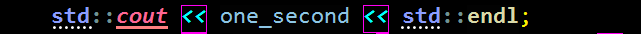
\includegraphics[width=\textwidth]{1.png}
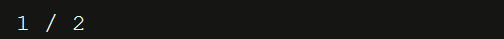
\includegraphics[width=\textwidth]{1-1.png}
\end{figure}

\begin{figure}[h]
	\caption{ Simplify the fraction}
	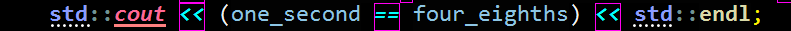
\includegraphics[width=\textwidth]{2.png}
	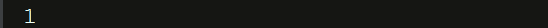
\includegraphics[width=\textwidth]{2-1.png}
\end{figure}

\begin{figure}[h]
	\caption{Basic Operator overload}
	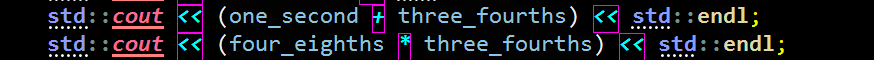
\includegraphics[width=\textwidth]{3.png}
	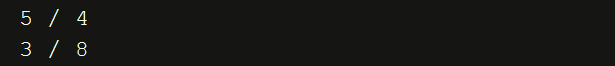
\includegraphics[width=\textwidth]{3-1.png}
\end{figure}


\begin{figure}[h]
	\caption{Relation Operator overload}
	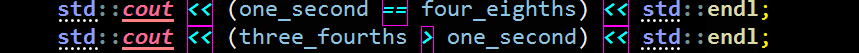
\includegraphics[width=\textwidth]{4.png}
	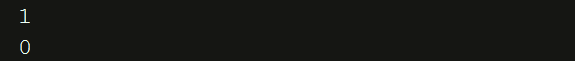
\includegraphics[width=\textwidth]{4-1.png}
\end{figure}


\begin{figure}[h]
	\caption{Input from stream}
	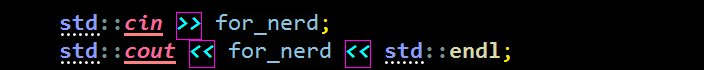
\includegraphics[width=\textwidth]{5.png}
	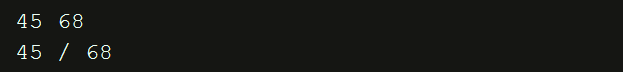
\includegraphics[width=\textwidth]{5-1.png}
\end{figure}

\begin{figure}[h]
	\caption{To double and string}
	
\includegraphics[width=\textwidth]{6.png}
	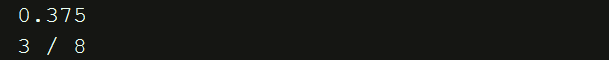
\includegraphics[width=\textwidth]{6-1.png}
\end{figure}

\newpage
\section{Features}
\begin{enumerate}
	\item Use C++ 11
	\item Simple exception handling
	\item Accurate compare
	\item GitHub repo :
	\href{https://github.com/HaoPatrick/oop}{https://github.com/HaoPatrick/oop} 
	\item That's all.
\end{enumerate}




\end{document}
